%
% Tikz Diagram
%

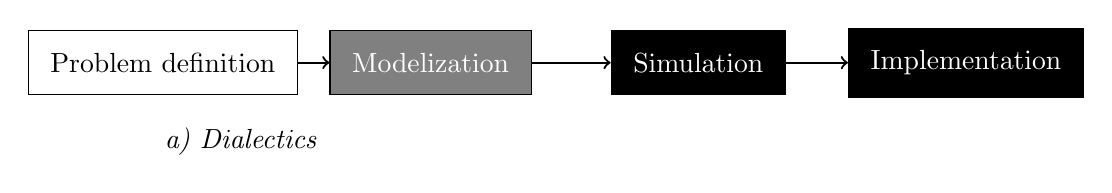
\begin{tikzpicture}

\tikzmath{
	\x = 3.2;
    \sx = \x + \x;
    \ssx = \sx + \x;
    \sssx = \ssx + \x;
}

\node[draw,inner sep=8pt] (prob) at (0,0) {Problem definition};
\node[draw,inner sep=8pt,fill=gray,text=white] (mod) at (3.4,0) {Modelization};
\node[draw,inner sep=8pt,fill=black,text=white] (sim) at (6.8,0) {Simulation};
\node[draw,inner sep=8pt,fill=black,text=white] (impl) at (10.2,0) {Implementation};

\draw[->,draw=black,thick] (prob) to (mod);
\draw[->,draw=black,thick] (mod) to (sim);
\draw[->,draw=black,thick] (sim) to (impl);

\node at (1.0, -1.0) {\textit{a) Dialectics}};

\end{tikzpicture}
